% ---------------------------- comment out when compiling the full document -------------------
\documentclass[twoside,12pt]{packages/mytustyle}  % default square logo 
\usepackage{amssymb}
\usepackage{caption}
\usepackage{upgreek}
\usepackage{subfig}
\usepackage{textcomp}

\usepackage{packages/fancyhdr}% http://ctan.org/pkg/fancyhdr
\pagestyle{fancy}% Change page style to fancy
\fancyhead[OR]{\renewcommand\thesection}
\fancyhead[ER]{\renewcommand\chaptername}

%\fancyhf{}% Clear header/footer
%\fancyhead{}
%\fancyhead[RO, LE]{Introduction}	
%\fancyhead[RO, LE]{\rightmark}	
%\fancyfoot{}
%\fancyfoot[RO, LE]{\thepage}% \fancyfoot[R]{\thepage}
\renewcommand{\headrulewidth}{0.7pt}% Default \headrulewidth is 0.4pt
%\renewcommand{\footrulewidth}{0.7pt}% Default \footrulewidth is 0pt
%\rfoot{\thepage}
\usepackage{lineno}
  \linenumbers 
 \usepackage{enumitem}
\setlist[description]{leftmargin=0cm,labelindent=0cm}
%
% \let\origdescription\description
%\renewenvironment{description}{
%  \setlength{\leftmargini}{0em}
%  \origdescription
%  \setlength{\itemindent}{0em}
%  \setlength{\labelsep}{\textwidth}
%}

{\endlist}

\begin{document}
\baselineskip=15pt
% ---------------------------------------------------------------------------------------------------------------



% ---------------------------------------------------------------------------------------------------------------
\chapter{Introduction}
% ---------------------------------------------------------------------------------------------------------------


The aim of the thesis is to present and discuss applications of diamond based particle detectors. 

The introductory chapter paints a picture of the current state of particle physics research. It presents some of the research institutes that are active in this field, pushing the boundaries of human knowledge further. It explains their goals and the means with which they are achieving them. Next section describes particle detectors in a broad sense -- their history and the types existing now. One type in particular -- a diamond detector -- is then described more in detail.

Second chapter discusses the properties of diamond detectors. Dissecting the detector chain into individual parts and describing them in detail -- sensors, amplifiers, digitizers and data processors. We learn about energy resolution in diamond, analog and digital noise contribution etc. Principles of signal formation are presented, starting with the famous Shockley-Ramo theorem and building from there. We will see that different types of radiation induce different electrical signals.

The base laid down in the second chapter is complemented in the third where the measurements are presented and the results discussed. The focus is on diamond's measurement stability with respect to irradiation damage. To carry out this study, two diamond sensors were irradiated to two different doses, with the measurements carried out before and after irradiation.

Building on the understanding of the behaviour of the diamond, two applications were developed. The fourth chapter describes the Diamond Beam Monitor, a detector that makes use of the diamond's charge measurement capabilities and its high radiation hardness. This detector has been installed in one of the largest particle physics experiments in the world and is currently taking data. Here, its development process is presented: the quality control procedures during assembly and installation, its performance in the test environment and some recent experimental data.

The final and most important chapter describes the real-time application for particle identification. Here the shape of the electrical signal of the diamond sensor is used to discriminate different types of radiation in real time and dead time free. The chapter includes the description of the device's logic and algorithms, lab test results and the application in neutron monitoring.


 




% ---------------------------------------------------------------------------------------------------------------
\clearpage
\section{Fundamental research}
\label{sec:fundphy}
% ---------------------------------------------------------------------------------------------------------------
This section gives a short overview of the institutes and collaborations carrying out fundamental physics research. The facilities were used for the research carried out in this thesis. 

The aim of fundamental (even pure or basic) research is to improve the scientific theories and verify them to improve our understanding of the universe.  It does not in itself focus on applying this research by developing products and is not meant to create a direct return on investment. Instead, it expands the overall knowledge of the human kind - by making the results freely available to the general public.

Particle physics research peers into the smallest constituents of the universe, dissecting the atoms into quarks and electrons, catching cosmic rays and figuring out what dark matter is made up of. Particle physicists want to explain the phenomena surrounding us by studying the fundamental particles and the mechanisms governing their interactions. By understanding this, we would be able to answer difficult questions; How did the universe begin? What is the invisible force (dark matter, dark energy) pushing the galaxies apart from each other? Where does mass come from? Why is there almost no antimatter in the universe? In this effort, scientists have formed several theories. One of them, the Standard Model of particles, is currently the best theory to describe the visible universe.

\begin{description}
\item[The Standard Model]
(SM) is a physics theory developed in the 1970's~\cite{Novaes:1999yn}. It was designed to explain the current experimental results. As such, it was also able to predict new discoveries and was a driving force for the scientists to invest time and money in developing new experiments. To date, it is by far the most established and verified physics theory. It explains how the basic building blocks of matter -- \emph{fermions} -- interact with each other via mediators of interactions called \emph{bosons}.  
\begin{figure}[!t]
\centering
\includegraphics[width=0.6\textwidth]{pics/sm}
\caption{Standard model \cite{Dominguez:2002395}}
\label{fig:sm}
\end{figure}
There are two main families of fermions - \emph{quarks} and \emph{leptons}, as shown in diagram~\ref{fig:sm}. Each group consists of six members divided into three \emph{generations}, the first being the lightest and most stable and the last the heaviest -- unstable. The nature around us is made up of the stable particles -- those from the second or third generations can only be found in cosmic rays or produced artificially using particle accelerators.

Quarks have a spin of 1/2 and a charge of either +2/3 (up, charm, top)  or -1/3  (down, strange, bottom) while the leptons have a spin of 1/2  and a charge of either 1 (electron, muon, tau) or 0 (electron neutrino, muon neutrino, tau neutrino). Leptons only exist individually -- they do not cluster. Quarks, however, immediately form a cluster of either two (unstable), three (more stable) or five (unstable). Two up and one down quark make up a proton whereas two down and one up quark make up a neutron.

In addition to fermions, each particle has a corresponding antiparticle -- a particle with the same mass but the opposite charge. If an antiparticle hits a particle, they annihilate each other, producing energy in form of photons. 

Bosons are the carriers of force, mediating weak (W$^+$, W$^-$ and Z bosons), strong (gluons) and electromagnetic (photons) interactions. The weak interaction is responsible for the radioactive decay of subatomic particles, thus playing an essential role in nuclear fission -- a process taking place in the stars. The electromagnetic interaction works at a macroscopic level -- it allows particles to interact via electric and magnetic fields. The strong interaction is effective at distances of a femtometer and it governs how quarks interact and bind with each other. An additional boson is the so-called Higgs boson and was discovered at CERN in 2012~\cite{}. It is a representation of the Higgs mechanism, which gives rise to the masses of all the particles in the Standard Model.
\end{description}

\subsection{CERN}
CERN (European Centre for Nuclear Research)~\cite{CERN:00000} is a nuclear research institute housing the largest particle physics laboratory in the world. It straddles the Swiss-French border just outside Geneva. It was established in 1954 to bring the war-torn Europe together by means of fundamental scientific research. Today, it has 22 member state countries and several observer states. More than 10000 scientists, engineers, technicians, students and others from all around the globe work at CERN on many projects in research fields ranging from particle to nuclear physics. The scope is to probe the fundamental structure of the universe and to understand the mechanisms governing it. Therefore CERN's main function is to provide the infrastructure for high-energy physics experiments. These are carried out using large machines called particle accelerators. These instruments boost beams of particles to high energies before making them collide with each other or with stationary targets. The resulting collisions are recorded by particle detectors and later analysed by physicists. To carry out research on the smallest constituents of matter, their dynamics and structure, very high energies are needed. This is why the most powerful accelerators are used for fundamental research. The largest accelerators at CERN are the Proton Synchrotron~\cite{}, the Super Proton Synchrotron~\cite{Mills:133232} and the Large Hadron Collider~\cite{}.

\subsection{Particle accelerators}
A particle accelerator is a machine that accelerates beams of charged particles like protons, electrons, ions etc. It generates electric fields that add kinetic energy to the particles, speeding them up. It then uses magnets to keep them within a defined trajectory. This can be either linear (linear accelerators) or circular (circular or cyclic accelerators). The advantage of the latter ones is that they can accelerate particles many times while keeping them in orbit.

Particle accelerators are used in numerous fields ranging from fundamental and material research, cancer treatment to industrial applications, such as biomedicine and material processing. There are several types of accelerators: electrostatic accelerators, linear accelerators (LINACs), cyclotrons, synchrocyclotrons, synchrotrons, synchrotron radiation sources and fixed-field alternating gradient accelerators (FFAGs).

\begin{description}
\item[The Large Hadron Collider]
(LHC, figure~\ref{fig:lhc}) at CERN is the largest particle collider in the world. It is a 27~km long circular machine set up in a tunnel deep under the surface (ranging from 50 to 175~m). It accelerates two proton beams to the energy of 6.5~TeV per beam before it makes them to collide with each other at four different points around its circumference. The LHC was build between 1998 and 2008 and was first successfully started in 2010 and operated stably until 2013 when it underwent a two years long upgrade. They restarted it at the beginning of 2015.
\begin{figure}[!t]
\centering
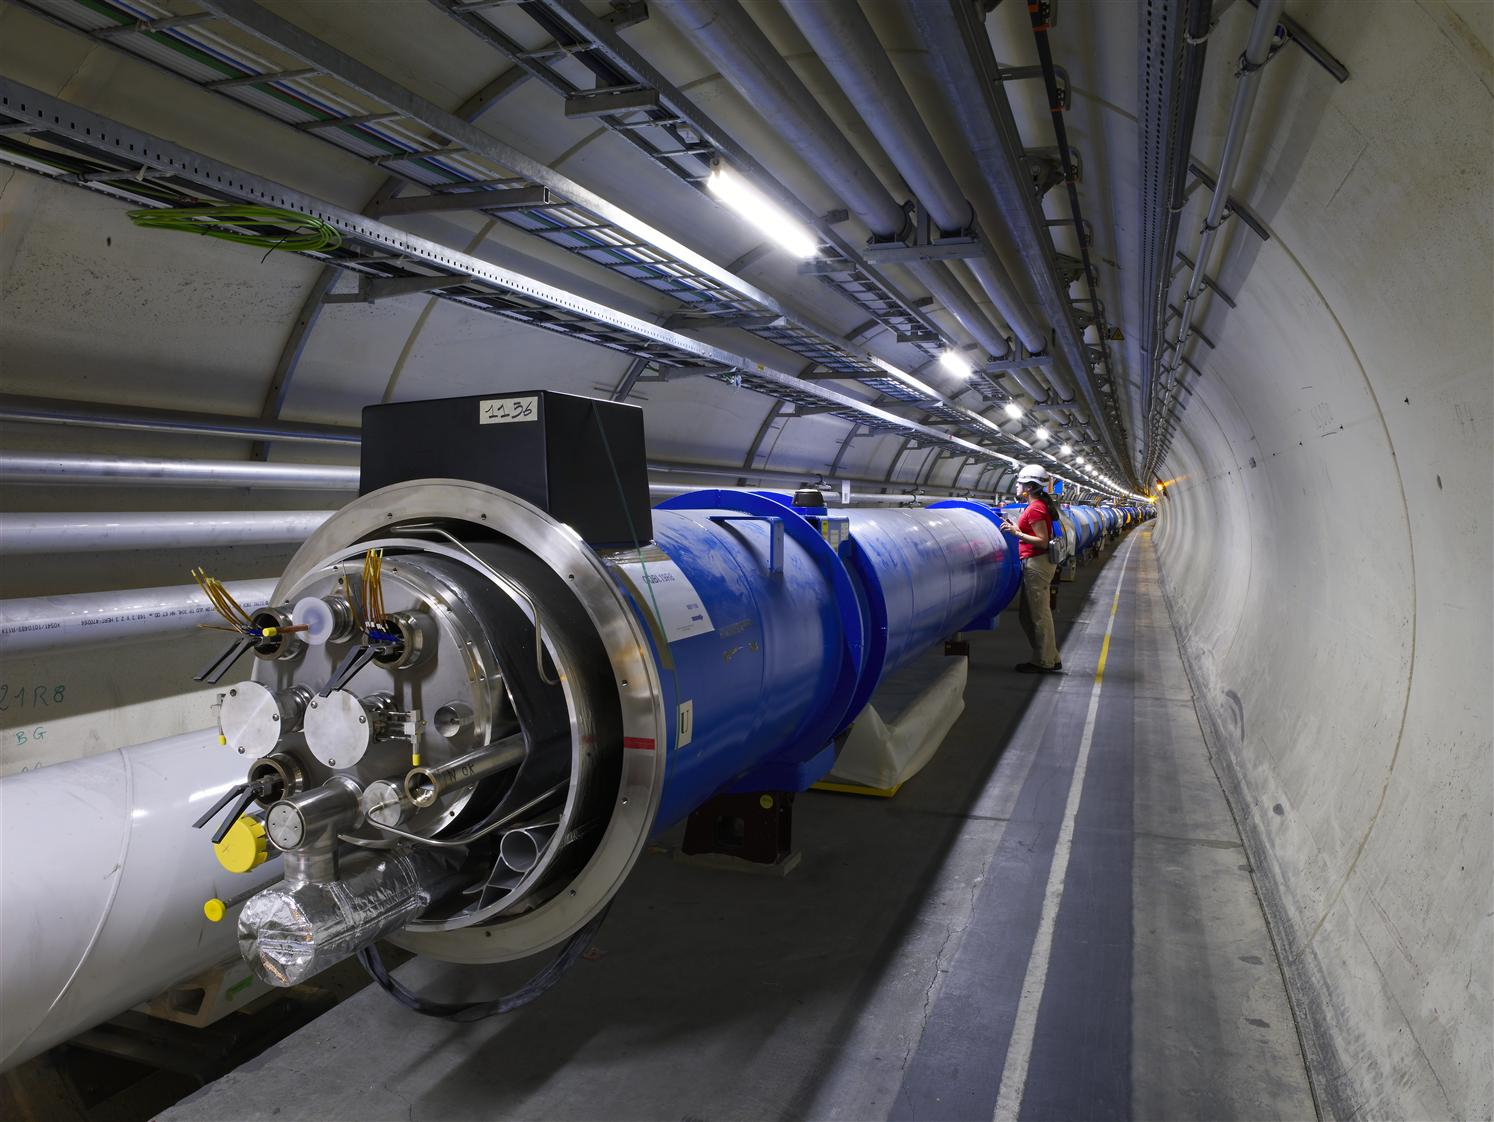
\includegraphics[width=0.6\textwidth]{pics/lhc}
\caption{The Large Hadron Collider \cite{Maximilien:1324852}}
\label{fig:lhc}
\end{figure}
The hair-thin particle beams travel inside two evacuated pipes with a $\sim$5~cm radius. Coils made up of a superconductive material are wound up around the pipes in special patterns. When they are cooled down to -271 \textdegree C using liquid helium, they become superconductive - the resistivity of the material drops significantly, minimising the heat dissipation despite high electric currents. These produce strong magnetic fields which bend the particles and keep them in a circular trajectory. The particles are accelerated when traversing the radiofrequency (RF) cavities with the RF frequency of 400~MHz. This oscillating frequency creates so-called buckets of bunches which are 2.5~ns long. Only one out of ten buckets is being filled, so the bunches are spaced at 25~ns. This defines the machine's clock as well as the maximum rate of collisions - the bunches travelling in the opposite direction will cross at the intersections up to 40~million times per second. Currently around 20 collisions occur during every crossing, making the maximum collision rate of $10^9$ per second. The number of collisions will further increase in the next years, when they will increase the number of particles in every bunch and decrease the transverse spread of the bunches -- squeeze them, therefore increase their density and the collision probability.
\end{description}

\subsection{The ATLAS experiment}
ATLAS (short for A Toroidal Lhc ApparatuS, figure~\ref{fig:atlas})~\cite{} is a particle physics experiment at CERN. Its purpose is to verify current theories and search for new discoveries by observing and analysing high energy proton-proton collisions produced by the LHC. It is the biggest experiment at CERN by dimensions (45~m in length and 26~m in height) and the number of people involved (more than 3000 physicists and engineers).
\begin{figure}[!t]
\centering
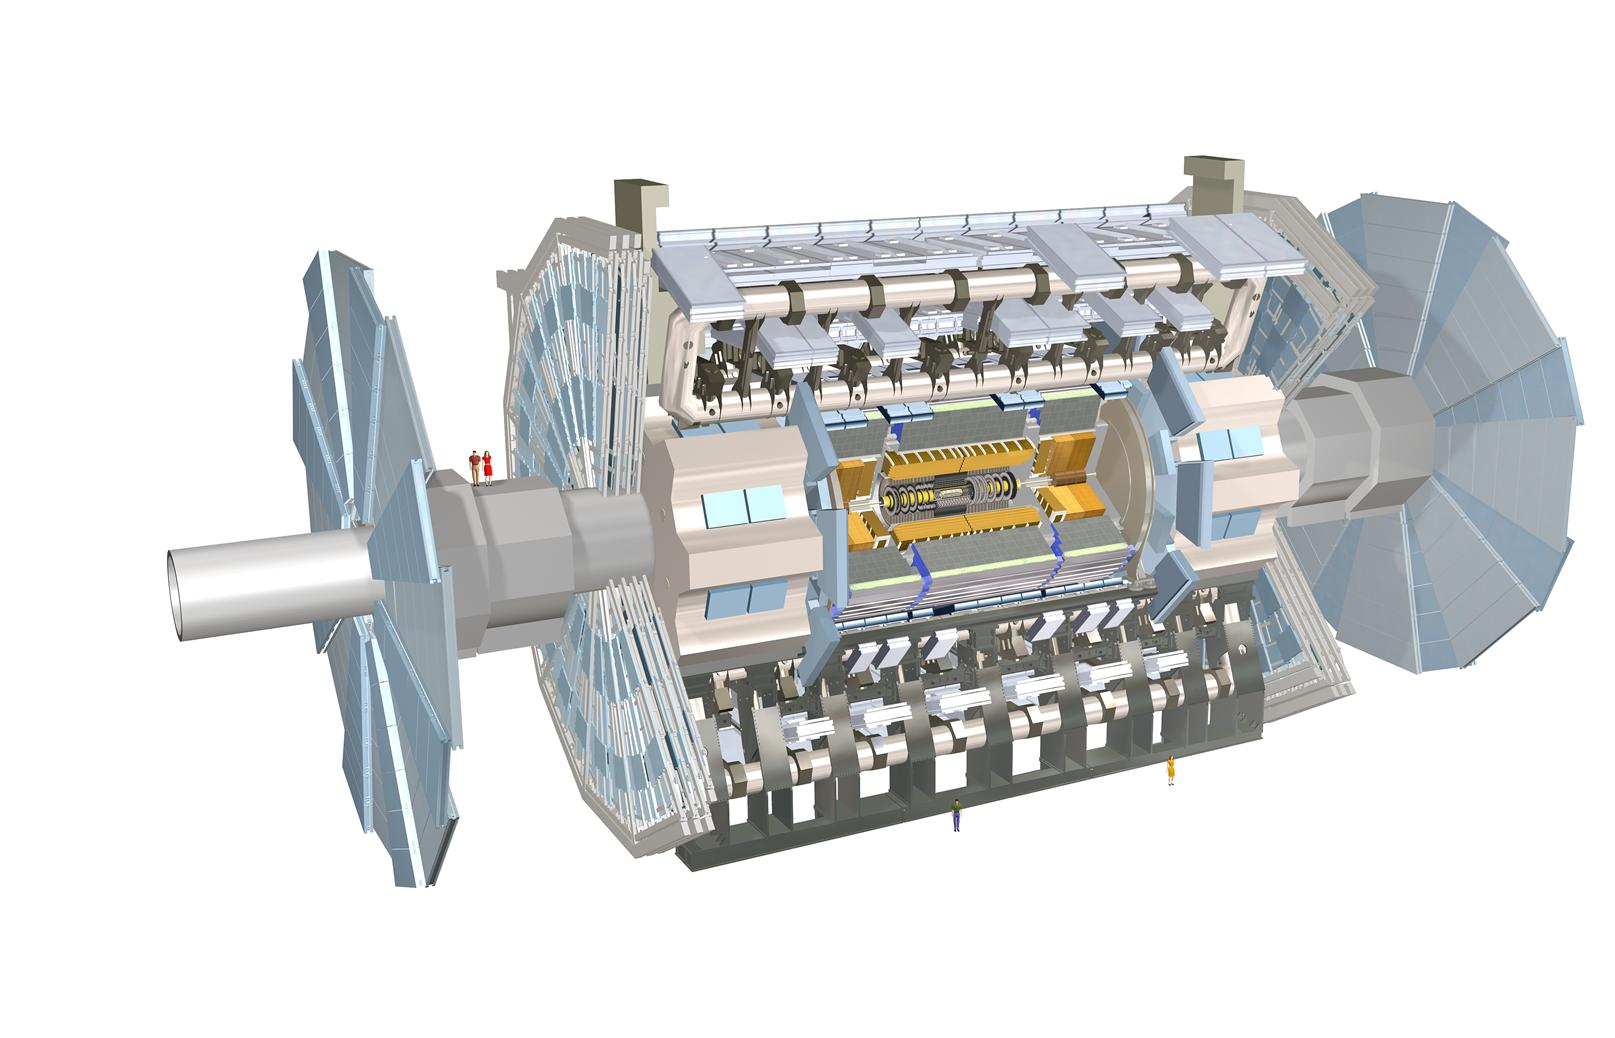
\includegraphics[width=0.8\textwidth]{pics/atlas3}
\caption{The ATLAS Experiment \cite{Pequenao:1095924}}
\label{fig:atlas}
\end{figure}
The ATLAS detector consists of many detectors, each designed to measure a specific property of the particles and photons produced during the collision. The closest to the collision point is the Inner Detector (ID), which consists of several layers of highly spatially segmented semiconductor sensors. These can record the path of the individual particles and photons. In addition, a strong magnetic field of 2~T curves the paths of the charged particles, which in turn allows the ID to identify an individual particle's charge and momentum. The next two parts are the electromagnetic and tile calorimeter. These detectors weigh a few thousand tonnes and measure the energy of the particles that are stopping in the bulk. The only particles that make it through the calorimeters are muons. These are detected by the Muon Spectrometer, a set of large plates placed all around the inner layers. Last is the superconductive magnet, which provides the magnetic field through the whole of ATLAS except the ID, which already has its own magnets. To sum up, the Inner Detector measures the charge and momenta of the particles and photons, the calorimeters measure their energies, the Muon Spectrometer measures muons and the magnets provide magnetic fields, which curve the trajectories of the charged particles, facilitating the charge and momentum measurements.

A complex Trigger and Data Acquisition system (TDAQ) is in place to distribute the clock signal, configure the detectors, trigger them and handle the output data.

The ATLAS detector has been designed to measure every collision taking place in its core. With 25~ns between collisions, this makes up 40~million collisions per second. In reality, the maximum rate is about 300~kHz. The recorded collision is called an event. Every event holds information from all the detector channels within ATLAS. With $\sim$$10^6$ channels, an event size is 10~MB. At the maximum achievable rate this means a data rate of up to 3~TB/s. Unfortunately no supercomputer existing today is capable of reading in and saving such a huge amount of data. This is where the trigger logic comes into play. It is programmed to decide in the order of tens of nanoseconds after an event whether this is a potentially interesting event or not. If so, it triggers the readout of the whole detector. This way, the recorded event rate is reduced from 300~kHz to $\sim$500~Hz, which is already within the limits of the computing centre's capabilities.


\subsection{Atominstitut, Vienna}
Atominstitut (ATI)~\cite{AtomInst:00000}, an institute for atomic and subatomic physics, was established in 1958 in Vienna as an inter-university institute. It currently houses around 200 people involved in a broad range of research fields: quantum, particle, neutron, nuclear, radiation and reactor physics, quantum optics etc. Its central facility is a TRIGA MARK II neutron reactor (described in detail below). 

As of 2002 the ATI is part of the University of Technology in Vienna.


\begin{description}
\begin{figure}[!t]
\centering
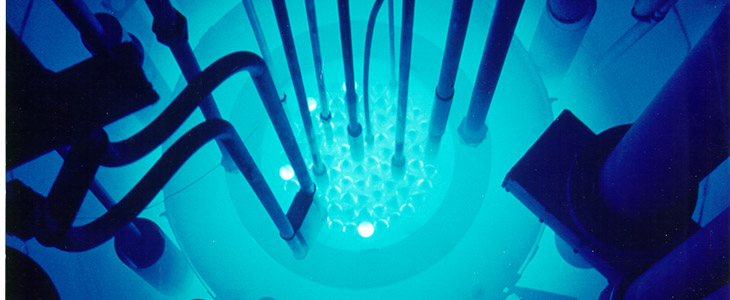
\includegraphics[width=0.8\textwidth]{pics/triga}
\caption{The TRIGA MARK II neutron reactor \cite{GeneralAtomics}}
\label{fig:triga}
\end{figure}
\item[TRIGA MARK II neutron reactor]~\cite{Triga:00000} is a reactor of a swimming-pool type used for training, research and isotope production. It is one of 40 such reactors worldwide, produced by an californian company General Atomic in the early 60's. It is capable of continuous operation at a maximum output power of 250~kW. 
The reactor core consists of 3~kg of 20~\% enriched uranium ($^{235}$U). The fuel moderator rods are mostly made up of zirconium with low percentage of hydrogen and uranium. Both the core and the rods are immersed in a pool of water as shown in figure~\ref{fig:triga} for the purpose of cooling and radiation protection. The surrounding concrete walls are 2~m wide with an added graphite layer for improved shielding. Four main experimental beam holes are placed radially through the walls. All exits are heavily shielded to prevent radiation damage to people, but still leaving enough space to set up experiments. Apart from the beam holes, there are several other exits and components, e.g. a thermal column for generation of thermal (low energetic) neutrons.


\end{description}

% MORE!



\subsection{n-ToF, CERN}
n-ToF (or neutron time-of-flight)~\cite{NTOF:00000} is a scientific collaboration with the aim of studying neutron-nucleus interactions. Over 30 institutes and universities are currently active members of this collaboration, among them Atominstitut in Vienna. n-ToF is also a facility at CERN where the experiments are carried out in a 200 m long experimental area. The knowledge stemming from the experimental results can then be applied in various fields ranging from nuclear technology and cancer therapy to astrophysics.

A pulsed beam of highly energetic protons (20~GeV/c) is produced by the Proton Synchrotron (PS) and aimed at a fixed lead spallation target. Each proton hitting the target produces around 300 neutrons of various energies. Initially highly energetic neutrons are slowed down by the target and by a slab of water placed behind it. This broadens their energy spectrum, which then ranges from meV (so-called thermal neutrons) to GeV (so-called fast neutrons). The neutrons are then collimated and sent through a 185~m long evacuated pipe to the experimental area, where they are made to collide with another target or a sample. The radiation resulting from the collisions is detected by a set of dedicated detectors around the interaction point (seen in figure~\ref{fig:ntof}). Having different energies, neutrons travel with different speeds, highly energetic ones reaching the target faster than those with low energies. Analysis of the collisions with a precise timing allows us to determine the interaction probability with sample material as a function of incident neutron energy.
\begin{figure}[!t]
\centering
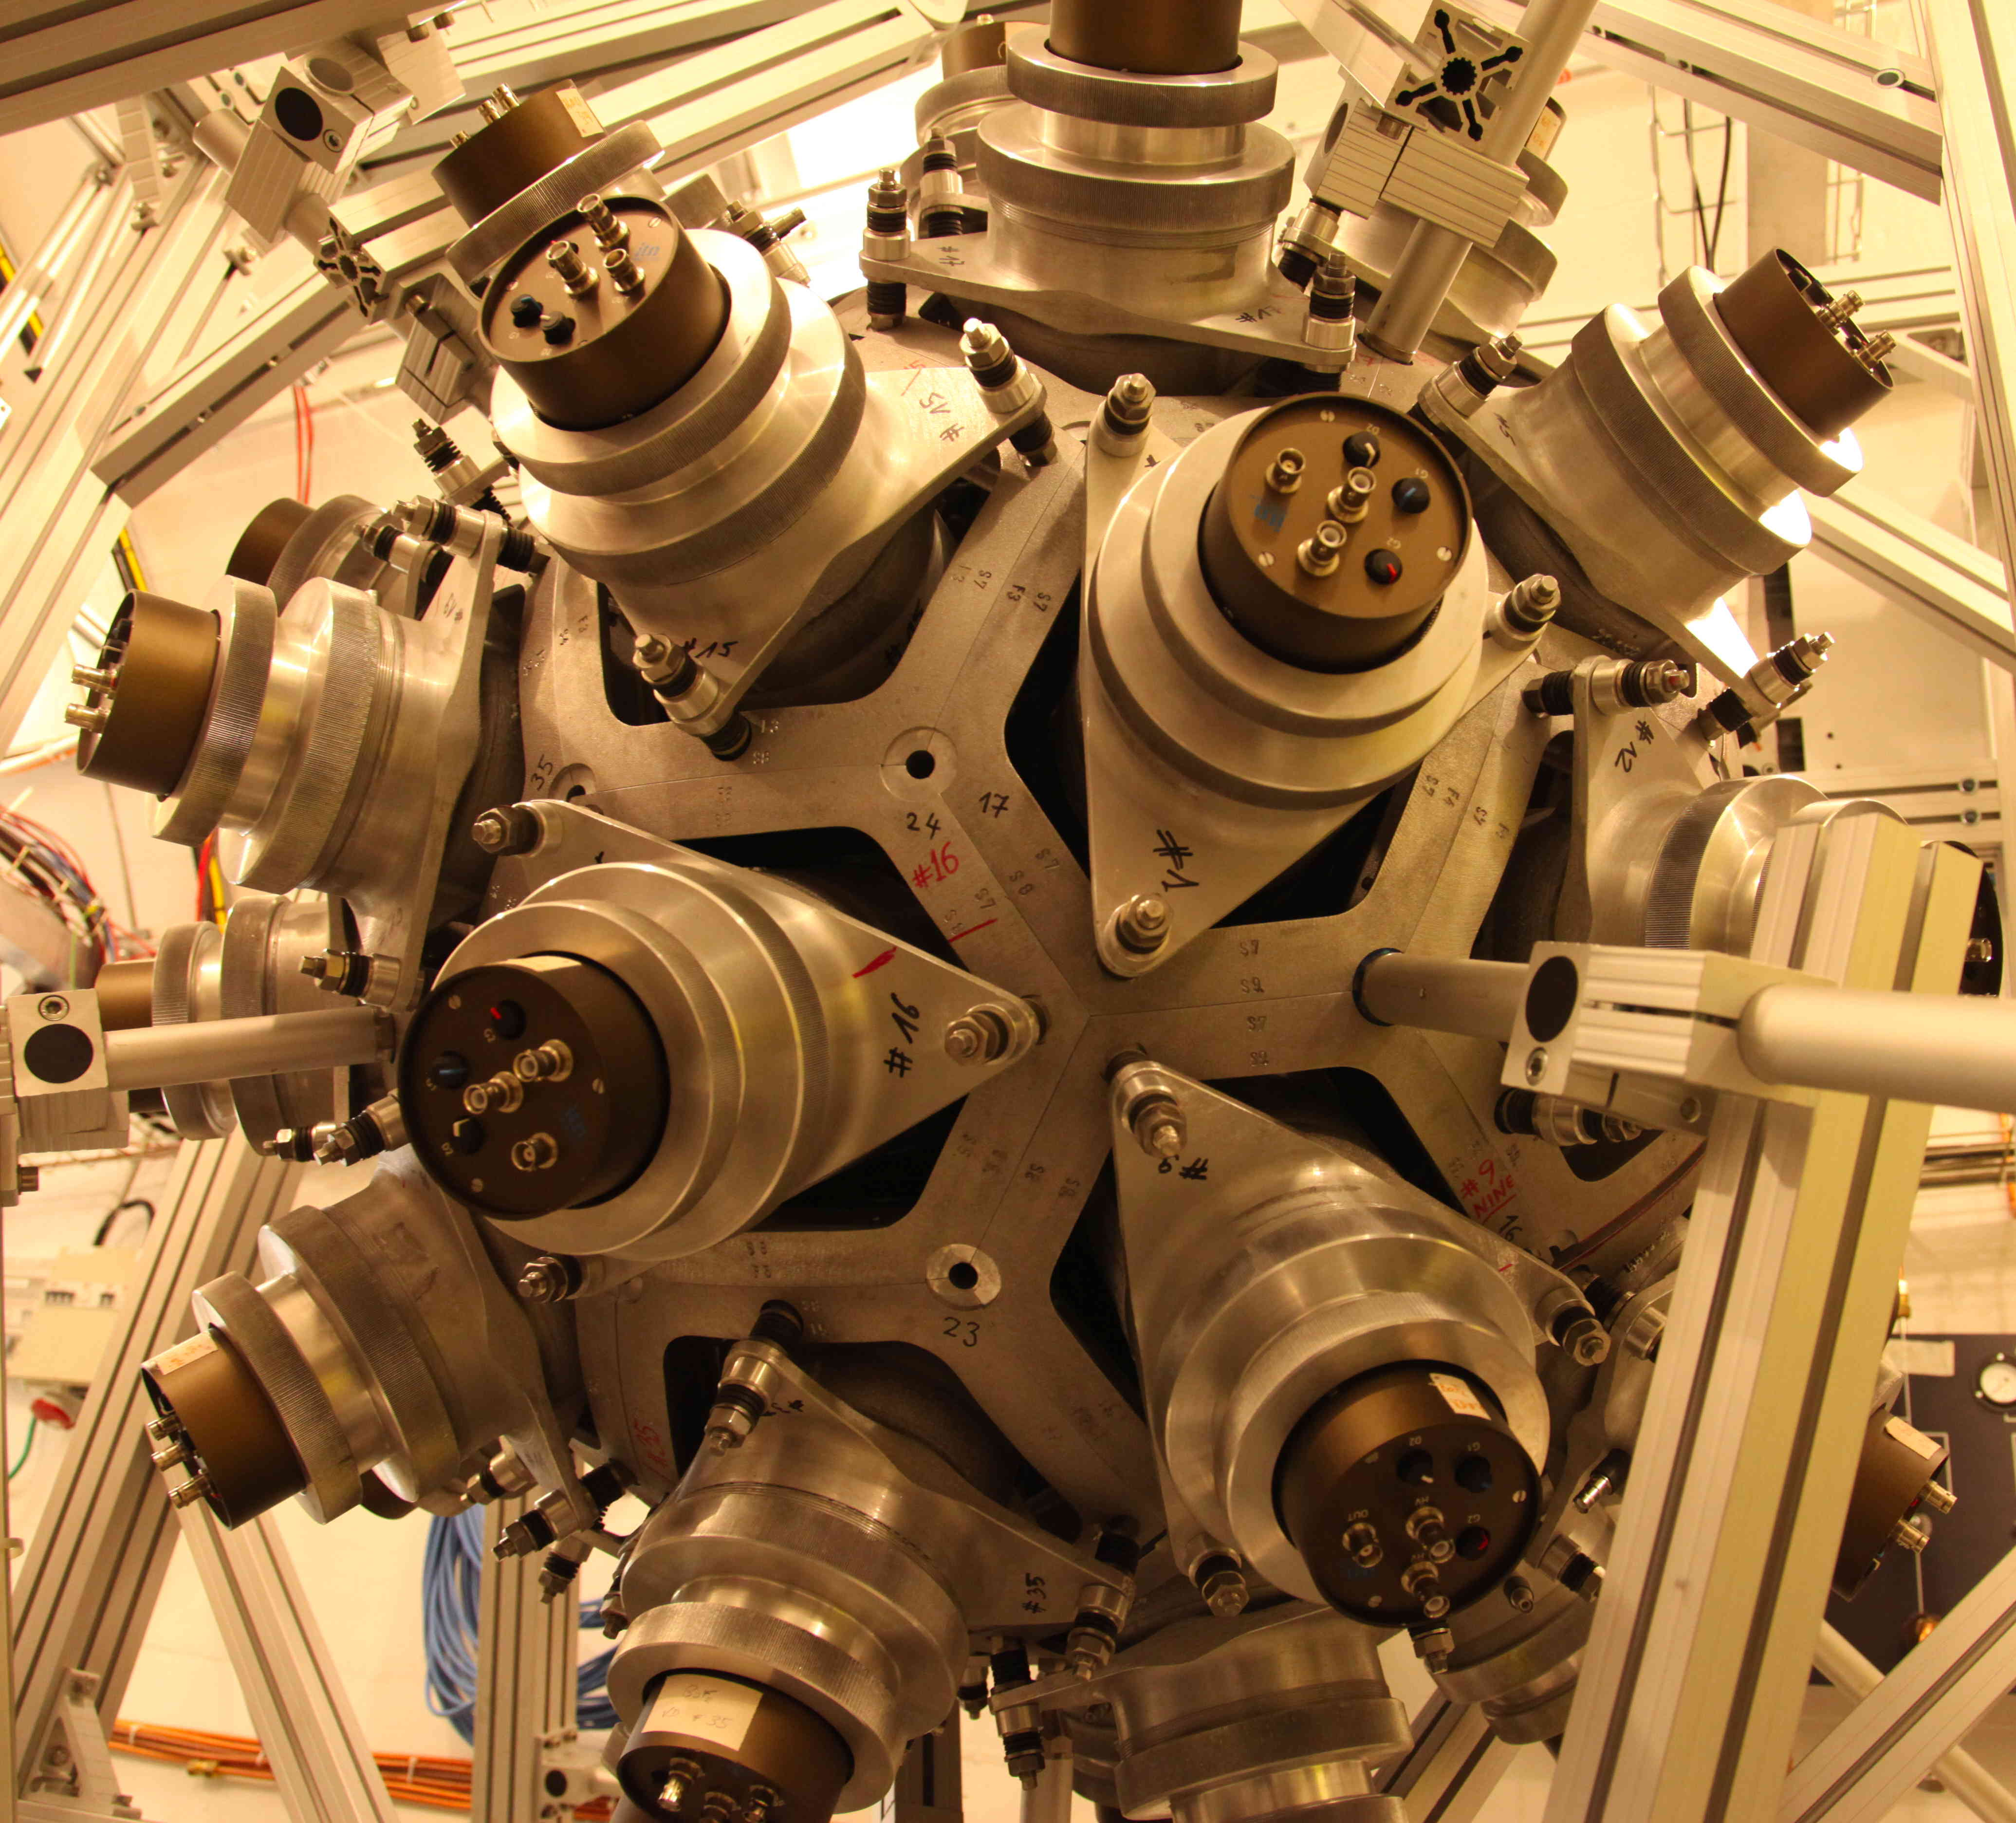
\includegraphics[width=0.6\textwidth]{pics/ntof}
\caption{The calorimeter in the n-ToF area \cite{Maximilien:1304589}}
\label{fig:ntof}
\end{figure}


% ---------------------------------------------------------------------------------------------------------------
\section{Particle detectors}
Particle detectors, or radiation detectors, have first come into use at the end of the 19th century. At that time Wilhelm R\"ontgen used a photographic plate onto which he shone X-rays. Soon after, in 1912, Victor F. Hess discovered cosmic rays during a balloon flight. This paved way for development of particle detectors. A cloud chamber was designed -- a chamber filled with a supersaturated vapour of water or alcohol. If a highly energetic particle traversed the chamber, the mixture ionised, creating condensation nuclei. These traces were visible and were photographed. All the subsequent particle detectors relied on the same principle of interaction between the particles -- ionisation. The bubble chamber invented in 1952 used a superheated transparent liquid -- a liquid heated just below its boiling point. A particle ionised the liquid, forming microscopic bubbles along its trajectory. Then followed the spark chamber and wire chamber where the particle ionised the gas, causing a spark between two parallel plates at a high potential difference. These are nowadays used in museums as showcases. Next were ionisation chambers, which measured the induced current of the free ionised charges moving in an externally applied electric field. Finally in the 1960s, semiconductor detectors were introduced. Their principle of operation is similar to that of an ionisation chamber, with the difference that a semi-conductive material is used as an ionisation medium instead of gas. Every technology has its advantages and disadvantages. Nowadays an ensemble of several types of detectors is used as a single detector system. There are many considerations that need to be taken into account when designing such a system: detector geometry, segmentation, event rate, efficiency, readout, support structures, cabling, cooling, cost etc.

On large, particle detectors can be divided in two groups: tracking detectors and calorimeters. The former are designed to measure trajectories (momentum) of particles and photons with a minimal impact on their flight path or energy. They must be built with a high spatial resolution and lightweight. Typically they are semiconductor detectors. The calorimeters, on the other hand, measure the energy of the particles/photons by stopping them. This means they need to be heavy and dense. A typical physics experiment nowadays would consist of a tracking detector enclosed by a calorimeter. This way both the momentum and energy are derived, measuring energy, charge and trajectory of every particle/photon.

%History and use (1 pg)
%Comparison table (2 pg)

%\subsection{Semiconductor sensors}

\subsection{Semiconductor detectors}
Semiconductor particle detectors are devices that use a semiconductor for detecting radiation. They work on the principle of an ionisation chamber. An incident particle or a photon ionises the atoms in the crystal lattice. The freed charges start drifting in an externally applied electric field, inducing current on the electrodes. The charges are freed if the deposited energy is higher than the energy band gap. There are many semiconductor materials currently existing, each with a different band gap. Germanium (Ge), for instance, has a band gap of 0.67~eV, which means that most of the electrons at the room temperature will already be in an excited state. Diamond's 5.5~eV band gap, on the other hand, is too high for the visible light to excite the electrons. However, silicon has been the material of choice for the majority of semiconductor applications, including radiation detectors. 
\begin{figure}[!t]
\centering
\includegraphics[width=0.6\textwidth]{pics/ibl}
\caption{The Insertable B-Layer -- a silicon particle tracker installed in the ATLAS experiment in 2014 \cite{MarcelloniDeOliveira:1702006}}
\label{fig:ibl}
\end{figure}
Semiconductor detectors are most widely used for tracking applications, like the Insertable B-Layer (see figure~\ref{fig:ibl})~\cite{Pernegger:1985432}, which was installed in ATLAS Experiment in 2014. They can be produced into light and thin sensors, they have a fast signal response, they are highly efficient and highly resistant to radiation damage. They also allow for a fine spatial segmentation to increase the tracking resolution. Semiconductor sensors come in several configurations. The simplest type is a pad -- a single plate measuring ~25~mm$^2$. Pads are used for particle counting and radiation monitoring. Next is a strip detector, a more finely segmented detector made out of long parallel sensing areas or strips. Each strip has its own signal line for readout. Usually the strip detectors are used in pairs -- one detector is placed on top of the other at a 90\textdegree~angle to increase spatial resolution in both axes. The third and the most finely segmented is a pixel detector, consisting of a 2D array of independent sensing areas. In tracking applications, pixel detectors are used where the detection resolution is the highest. Due to their high production cost and a high number of signal channels, they can only cover limited areas. Strip detectors are cheaper to produce and can be used to cover larger areas in several consecutive layers.

\subsection{Diamond sensors}
Diamond has been known for over two millennia, valued for its mechanical properties and its appearance. When we learnt how to synthesise it, diamond found its way to a broad range of industries which exploited its optical and electrical properties. The discovery of the Chemical Vapour Deposition (described below) as a new synthesis process gave rise to a range of new applications. From being used on machines for drilling tunnels it found its way to electronics, high-power switching devices, electrochemical systems, radiation sensors, quantum computing etc. Recently it was found that it also exhibit superconductivity. This thesis focuses on the use of diamond for radiation detection.
\begin{figure}[!t]
\centering
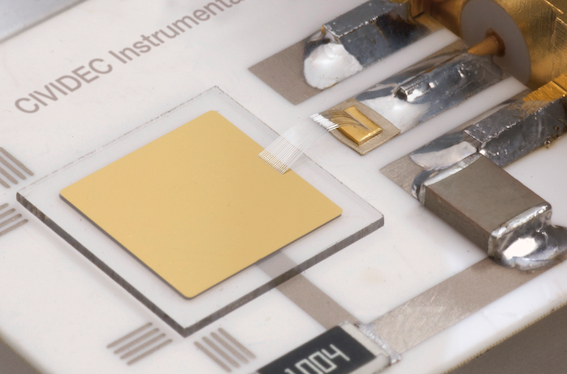
\includegraphics[width=0.6\textwidth]{pics/cividecpcvd}
\caption{A pCVD diamond pad detector \cite{Cividec:00000}}
\label{fig:cividecpcvd}
\end{figure}
Compared to a natural diamond, a detector-grade CVD diamond has almost no impurities (foreign atoms like nitrogen or boron). The carbon lattice is very uniform, which improves its electrical properties. It is an almost perfect insulator, but behaves as a semiconductor under certain conditions. Compared to silicon, the most widely used semiconductor material for radiation detection, it has many advantages, which are described in detail in chapter~\ref{}. Figure~\ref{fig:cividecpcvd} shows a diamond pad detector produced by CIVIDEC Instrumentation GmbH.
%Its energy band gap is three times as large, reducing the noise and  

\begin{description}
\item[Chemical vapour deposition] (CVD) is a process where a material is deposited from a gas onto a substrate, involving chemical reactions. It is often carried out under high pressure and high temperatures. It takes place in enclosed chambers called furnaces with careful regulation of the temperature, pressure and gas mixture. Synthetic diamond is grown at 700--900 \textdegree C with a mixture of hydrogen and methane gas. At this temperature the molecules dissociate into carbon and hydrogen atoms. The carbon atoms are the building blocks and are deposited on the surface of the substrate. However, they would rather form graphitic bonds as they are more stable than diamond bonds. Nevertheless, with high pressure, high temperature and with the abrasive atomic hydrogen, the graphitic double bonds are broken up and converted into diamond bonds. The speed of the growth can be anywhere between 0.1 and 10 micron per hour. The detector grade samples are grown at a rate of the order of 1 micron per hour. They can grow up to several millimetres in thickness. Their width, however, depends entirely on the substrate used. Diamond can be deposited on various materials: diamond, silicon, tungsten, quartz glass etc. The substrate material must be able to withstand the high temperatures during the CVD process. The diamond substrate does not need any surface pre-treatment. Carbon atoms form bonds with atoms in the existing crystal structure. This is a so-called homoepitaxial growth where the newly deposited atoms retain the orientation of the structure in the substrate. Other non-diamond substrates, however, need to be pre-treated, usually by being polished using diamond powder. Some powder particles remain on the surface, acting as seeds for the growth of small crystals or grains. These grains grow and at some point merge with the adjacent ones, making up a compact material. The lower side is later polished away. These diamonds are called \emph{polycrystalline} (pCVD) whereas those grown on a diamond substrate are \emph{single crystal} (sCVD) diamonds. The area of the former can be large - up to 0.5~m$^2$ or more compact 15~cm$^2$ in the case of detector grade diamonds. The sCVD diamonds, on the other hand, can currently only measure up to 1.5 cm$^2$.
\end{description}




\bibliography{bib1}{}
\bibliographystyle{plain}



%
%\begin{thebibliography}{9}
%
%\bibitem{bib01}
%G. Aad et al., \emph{The ATLAS Collaboration}, 2008 JINST 3 S08003, DOI: 10.1088/1748-0221/3/08/S08003.
%
%%radiation hardness
%\bibitem{bib51}
%M. Miku\v{z} et al., \emph{Diamond sensors in HEP}, 2012, PoS(ICHEP2012)524.
%
%%cited
%\bibitem{bib8}
%E. Griesmayer, B.~Dehning, \emph{Diamonds for beam instrumentation}, TIPP 2011.
%
%%cited
%\bibitem{bib12}
%M. Capeans et al., \emph{ATLAS Insertable B-Layer Technical Design Report}, 2010, CERN-LHCC-2010-013. ATLAS-TDR-19.
%
%\end{thebibliography}


% ---------------------------- comment out when compiling the full document -------------------
\end{document}
% ---------------------------------------------------------------------------------------------------------------
